\chapter{Nuclear Data}

\fancyhead[L]{University of Surrey, November 2026 \hfill Professor David Jenkins}
\label{nucdat}
\section{Introduction}
The following notes are based on \textit{Nuclear Data: A Primer} by Jenkins and Wood in preparation for the PLANET baseline training lectures in nuclear structure. Including additions from Krane, \textit{Nuclear Physics in a Nutshell} by Bertulani, chapters 3, 9 and 11 of \textit{A Modern Primer in Particle and Nuclear Physics} by Terranova, third year Nuclear II lecture notes (Andreyev) and fourth year Quantum V lecture notes (Wilson-Rae/Cavill).

\section{Nuclear Data Sets}
Nuclear data are mostly organised by mass chains or \(A\) chains i.e. data is evaluated for nuclear isobars (sometimes an \(A\) chain will contain a single isotope). Recall that there are various categories of isotopes - groups of nuclei that share a common property:
\begin{itemize}
    \item Isobar: Same mass, \(A = N + Z\).
    \item Isotope: Same proton number, \(Z\).
    \item Isotone: Same neutron number, \(N\).
    \item Isomer: Same mass and proton number, but with some nucleons in an excited state e.g. metastable Technetium-99, \ce{^{99m}Tc}.
\end{itemize}
Instead of \(A\) chains, groups occassionally produce `horizontal' compilations and evaluations i.e. a compilation or evaluation of a specific nuclear property across an entire range of \textit{A}, \textit{Z} and \textit{N} - referred to as a mass surface. An example of a horizontal compilation is that of nuclear masses, maintained by the Atomic Mass Evaluation (AME) network. 
Examples of commonly used nuclear databases:
\begin{itemize}
    \item Evaluated Nuclear Structure Data File (\ensdf) and Experimental Unevaluated Nuclear Data List (\xundl) maintained by the National Nuclear Data Centre (NNDC). It also publishes evaluations by \(A\) chain in the journal \href{https://www.sciencedirect.com/journal/nuclear-data-sheets}{\textit{Nuclear Data Sheets}} and has an interactive plotting tool, \href{https://www.nndc.bnl.gov/nudat3/}{NuDat3}.
    \item Specialised evaluations appear in journals such as \href{https://www.sciencedirect.com/journal/atomic-data-and-nuclear-data-tables}{\textit{Atomic Data and Nuclear Tables}} and \href{https://iopscience.iop.org/journal/1674-1137}{\textit{Chinese Physics C}}. Review articles on special topics appear in \href{https://www.sciencedirect.com/journal/physics-reports}{\textit{Physics Reports}}, \href{https://www.sciencedirect.com/journal/progress-in-particle-and-nuclear-physics}{\textit{Progress in Particle and Nuclear Physics}}, \href{https://iopscience.iop.org/journal/0034-4885}{\textit{Reports on Progress in Physics}} and \href{https://journals.aps.org/rmp/}{\textit{Reviews of Modern Physics}}.
\end{itemize}

\section{Gross Properties of Nuclei}
Gross properties are those which involve the entire nucleus - radius and mass fall within this definition. 

\subsection{Measuring Radii}
A nucleus doesn't have a sharp surface - it is diffuse. This is deduced from inferring charge density distributions, \(\rho(r)\), using elastic electron scattering. Charge density as a function of the distance from the centre of the nucleus obeys a typical Fermi distribution.

\[\rho (r) = \frac{\rho_0}{1+e^{r-\frac{R_{1/2}}{a}}}\]

Where \(\rho (R_{1/2})=\frac{1}{2}\rho_0\) and \(a\) gives the width of the surface diffuseness. The width of the interval where density decreases from 90\% of \(\rho_0\) to 10\% of \(\rho_0\) is \(4.4a\). These diffuse effects are mainly due to p-n interactions. Nucleon density is approximately constant inside the nucleus. For most nuclei, there are more neutrons than protons so the individual density distributions would both follow the same shape of a Fermi distribution, but the proton curve would be lower. 

Instead of electron scattering, x-ray spectroscopy be used on muonic atoms to provide further information on the density distribution. With their increased mass, muons exist closer to the nucleus than electrons so a higher fidelity is possible.

\subsubsection*{RMS Charge Radius and Isotope Shifts}
Since nuclear surface diffuseness is not a fixed geometric property, it is convenient to define an rms charge radius, \(\langle r^2 \rangle ^{1/2}\), for a given nuclear species (a given \(Z\) and \(N\)). This is a well-defined quantity and is unique for each nuclear species. These data are usually plotted as isotope shifts - small variations in charge radius along isotopic chains (measured using optical hyperfine spectroscopy), between a given nucleus and a specified isotope of that nucleus i.e. they are plotted for a fixed \(Z\) as a function of \(N\).

When \(\langle r^2 \rangle ^{1/2}\) values are plotted as a function of \(A\), they follow the liquid drop model closely. Following:
\[\left[\frac{5}{3}\langle r^2\rangle\right]^{1/2}=R_0 A^{1/3}\]

\begin{figure}[H]
\captionsetup{width=.75\textwidth}
    \centering
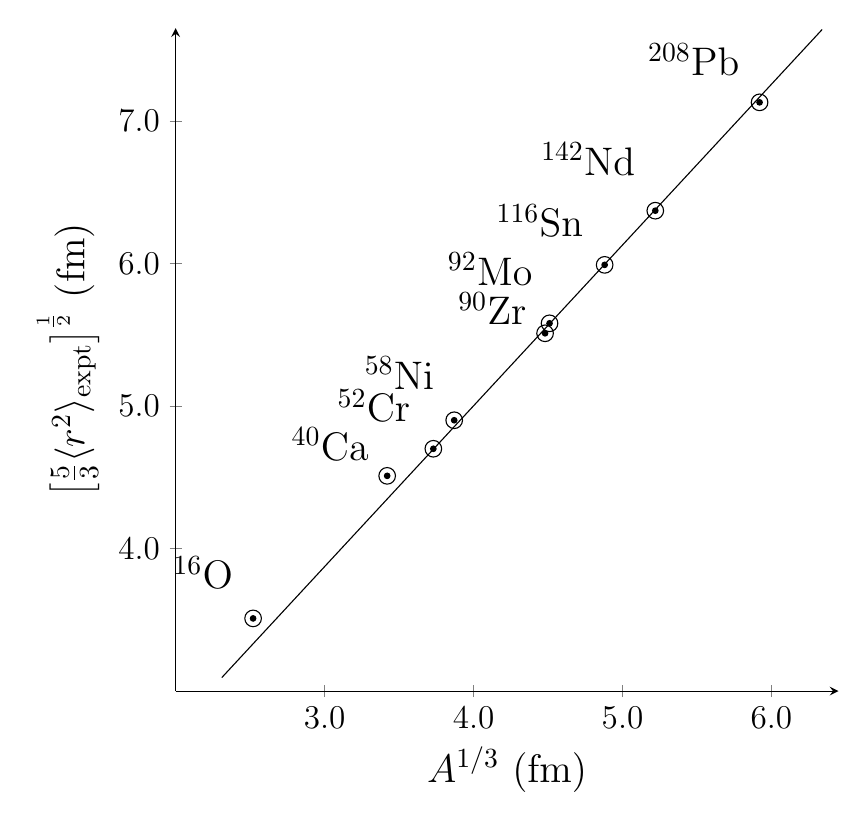
\begin{tikzpicture}
\begin{axis}[
    width=10cm, height=10cm,
    axis lines=left,
    xmin=2, xmax=6.45,
    ymin=3, ymax=7.65,
    xtick={3.0,4.0,5.0,6.0},
    ytick={4.0,5.0,6.0,7.0},
    yticklabel style={/pgf/number format/fixed, /pgf/number format/fixed zerofill, /pgf/number format/precision=1},
    xticklabel style={/pgf/number format/fixed, /pgf/number format/fixed zerofill, /pgf/number format/precision=1},
    xlabel={$A^{1/3}$ (fm)},
    ylabel={$\left[\frac{5}{3}\langle r^2\rangle_{\mathrm{expt}}\right]^{\frac{1}{2}}$ (fm)},
    xlabel style={font=\Large},
    ylabel style={font=\Large},
    tick label style={font=\large},
    clip=false,
]

% Straight-line guide
\addplot[black, thin, domain=2.31:6.34] {1.128*(x-2.31)+3.095};

% Data points (circled dots)
\addplot[only marks, mark=*, mark size=1pt] coordinates {
    (2.52,3.51) (3.42,4.51) (3.73,4.70) (3.87,4.90)
    (4.48,5.51) (4.51,5.58) (4.88,5.99) (5.22,6.37) (5.92,7.13)
};
\addplot[only marks, mark=o, mark size=3pt] coordinates {
    (2.52,3.51) (3.42,4.51) (3.73,4.70) (3.87,4.90)
    (4.48,5.51) (4.51,5.58) (4.88,5.99) (5.22,6.37) (5.92,7.13)
};

% Nuclide labels
\node[anchor=south east, font=\Large] at (axis cs:2.45,3.65) {$^{16}$O};
\node[anchor=south east, font=\Large] at (axis cs:3.36,4.55) {$^{40}$Ca};
\node[anchor=south east, font=\Large] at (axis cs:3.64,4.82) {$^{52}$Cr};
\node[anchor=south east, font=\Large] at (axis cs:3.80,5.05) {$^{58}$Ni};
\node[anchor=south east, font=\Large] at (axis cs:4.42,5.50) {$^{90}$Zr};
\node[anchor=south east, font=\Large] at (axis cs:4.46,5.78) {$^{92}$Mo};
\node[anchor=south east, font=\Large] at (axis cs:4.80,6.12) {$^{116}$Sn};
\node[anchor=south east, font=\Large] at (axis cs:5.15,6.55) {$^{142}$Nd};
\node[anchor=south east, font=\Large] at (axis cs:5.85,7.25) {$^{208}$Pb};

\end{axis}
\end{tikzpicture}
    \caption{Nuclear rms charge radii compared to the liquid drop model. 
    Almost exact for \(A\geq90\), deviation for \(A < 90\) due to surface 
    diffuseness. Adapted from fig. 1.7 in \textit{Primer} \anth}
    \label{rms_vs_A}
\end{figure}



Figure \ref{rms_vs_A} shows that nuclear size scales with \(A\). If the nuclear binding force were long ranged and attractive, the size of a nucleus would shrink with a larger number of nucleons due to the increased binding. This is what happens for atoms, due to the long ranged Coulomb attraction between the \(+Ze\) charge of the nucleus and the electrons. 

\subsection{Measuring Masses}
Masses are usually measured for atoms, whereas radii are measured for nuclei. Atoms are easier to handle than nuclei, producing a bare nucleus would involve stripping away all electrons leaving a highly charged ion which would be neutralised by capturing electrons from its environment. Instead, singly charged ions are used because they are easy to maintain and manipulate under a vacuum with E and B fields. 

\subsubsection*{Nuclear vs Atomic Binding Energy}
The mass of a nucleus is less than the mass of its constituent parts due to binding energy. Binding energy is on the order of 1\% the mass of the total nucleus. For an atom, masses also include the mass of the electrons minus the electronic binding energy. However, electronic binding energy is comparatively very small, less than the measurement uncertainty of the total atomic mass (note that this does not mean atomic binding energy is unknowable, it can be inferred by summing ionisation potentials for successive removal of the electrons in a given atom). Hence, we only consider nuclear binding energy, \(B(Z, N)\).

\[M(Z, N) = Zm_p + Nm_n + Zm_e - B(Z, N)\]

\subsubsection*{Binding Energy per Nucleon}
Binding energy alone, when plotted against \(A\) is monotonic. However, plotting binding energy per nucleon, \(B/A\), we make the following observations. 
\begin{enumerate}
    \item The vast majority of nuclei, \(20 < A < 200\) have an almost constant binding energy per nucleon, \(8.3 \pm 5\%\) MeV/nucleon.
    \item Maximum \(B/A\) occurs at \ce{^{62}Ni}.
    \item There is a steep decline in \(B/A\) down to the lightest nuclei.
    \item There is a steady and slowly steepening decline in \(B/A\) toward heavy nuclei.
\end{enumerate}
We can make the following interpretations of the above observations.
\begin{enumerate}
    \item \textbf{Constancy of B/A Beyond \ce{^{62}Ni}}: The force binding nucleons must be short ranged as it will mostly only influence its nearest neighbours, resulting in a saturation of the binding i.e. there can only be so many neighbours of a given nucleon. This is analogous to water having a constant boiling point (\(L_v\)) at STP, no matter the amount of water being heated. If the binding force were long ranged and attractive, binding energy would be non-linear and increasing. 
    \item \textbf{Maximum Value of B/A}: A result of the balance between the minimum surface-area-to-volume ratio and the minimum Coulomb repulsion between protons. The occurence at \ce{^{62}Ni} is coincidentally near where stellar fusion stops, but it does not mark a profound nuclear property. 
    \item \textbf{Steep Decline in B/A for Light Nuclei}: Also a consequence of the short range of the strong nuclear force. In light nuclei, almost all nucleons are at the surface, hence they do not have a full set of neighbours as most nucleons do in a heavy nucleus. So, the binding energy of a light nucleus is unsaturated.
    \item \textbf{Slow Decline in B/A for Heavy Nuclei}: A long ranged and repulsive force would result in binding energy being non-linear and decreasing - seen in heavy nuclei because of the increasing number of protons and their long ranged Coulomb repulsion.
\end{enumerate}

\newpage
\section{Differences in Radii and Masses}
\subsection{Neutron Separation Energies}
By plotting differences in gross properties, shell structure becomes apparent. Figure \ref{isotopicshift} shows marked increase in isotope shifts at magic numbers.

\begin{figure}[H]
    \centering
    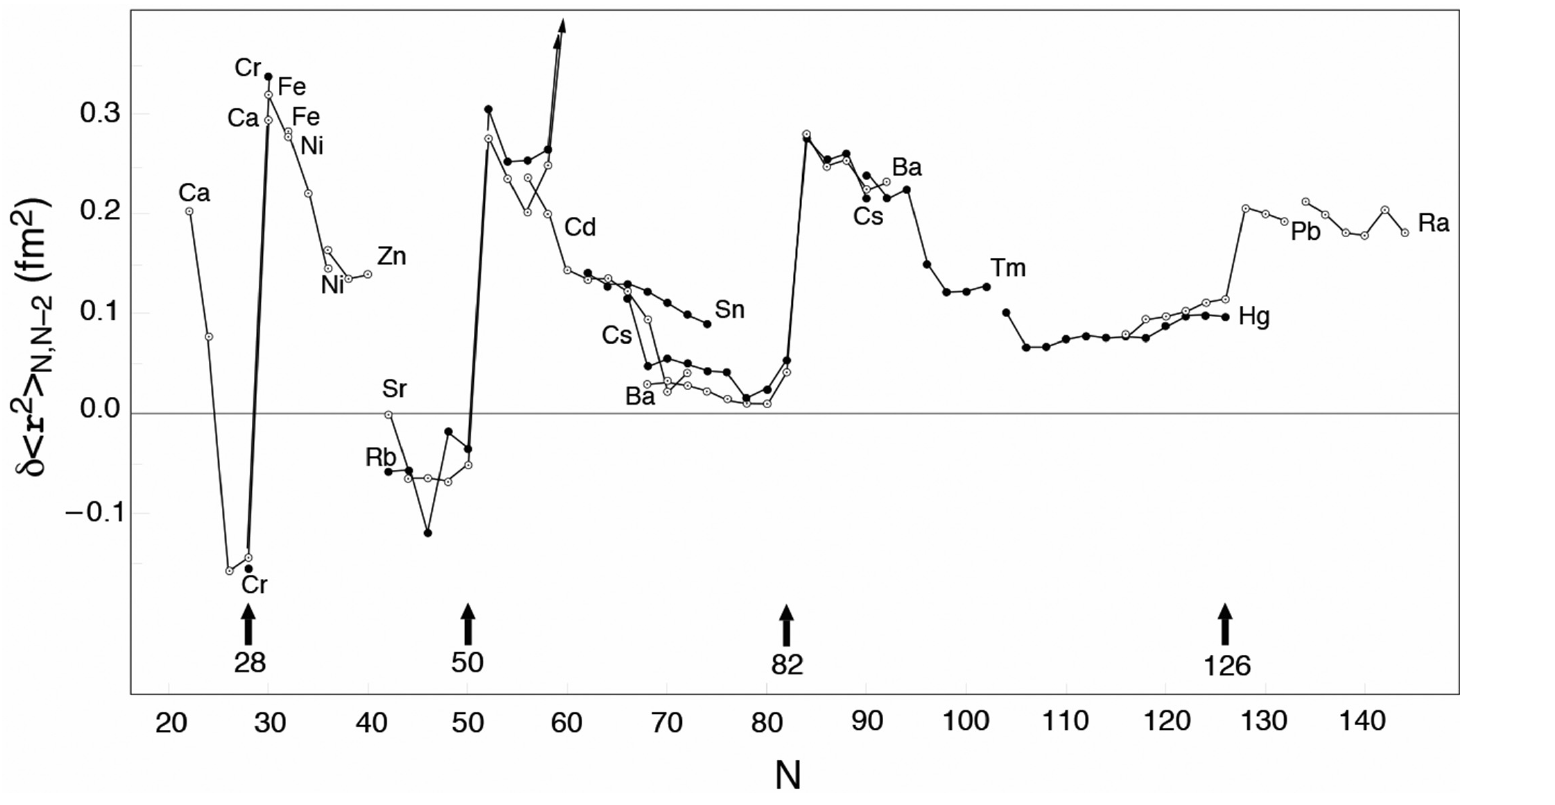
\includegraphics[width=0.8\textwidth]{assets/2.1.2 isotope_shifts.png}
    \caption{Isotope shifts for specific isotopic sequences of nuclei. Fig. 1-9 of \textit{Primer}.}
    \label{isotopicshift}
\end{figure}

Differences in binding energies are termed separation energies. One-neutron separation energy is defined as:
\[S_n = -M(A,Z,N) + M(A-1,Z,N-1)+m_n\]

Observations to note from figure \ref{Sn}:
\begin{itemize}
    \item Odd-even staggering of \(S_n\).
    \item Discontinuities, `steps' down, with increasing \(N\) or \(A\).
    \item Between the steps, the trend is smooth and down-sloping with increasing \(N\) or \(A\).
\end{itemize}

\begin{figure}[H]
    \centering
    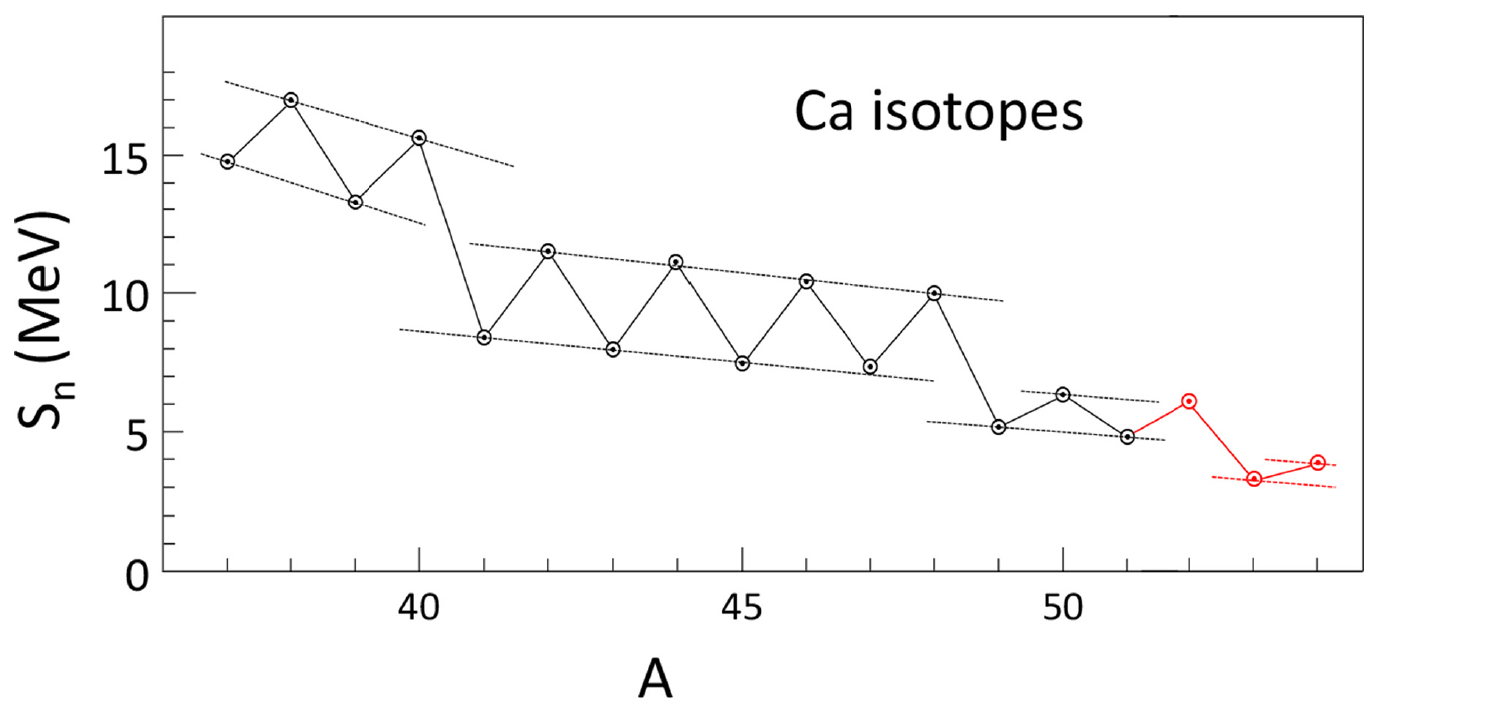
\includegraphics[width=\linewidth]{assets/2.1.3 Sn.png}
    \caption{One-neutron separation energies. Data from \href{https://amdc.impcas.ac.cn/}{\ul{AMDC}} files. Fig. 1.10 \textit{Primer}.}
    \label{Sn}
\end{figure}


We can make the following interpretations of the above observations.
\begin{itemize}
    \item \textbf{Odd-even Staggering}: Due to enhanced binding when the neutron number is even. Similarly observed for \(S_p\). An effect termed pairing. Manifestation of quantum mechanical correlations.
    \item \textbf{Steps Down}: Due to `shell closures'. From left to right in the figure, successive neutrons are removed. Nucleons are confined in an average potential generated by all of the other nucleons. Nucleons sequentially fill orbitals. When an energy gap is reached in the removal process, there is a sudden step up in the removal energy. This effect is more clearly seen for two-neutron separation energies, figure \ref{2Sn}.
    \item \textbf{Sloping Down Between Steps}: Due to the confining potential changing with \(\sim A^{1/3}\). As \(A\) increases, potential width increases and the potential becomes shallower.
    \item \textbf{Shell Closure Locations}: Only occur at the classical magic numbers, 20, 28, 50, 82, 126.
\end{itemize}

\begin{figure}[H]
    \centering
    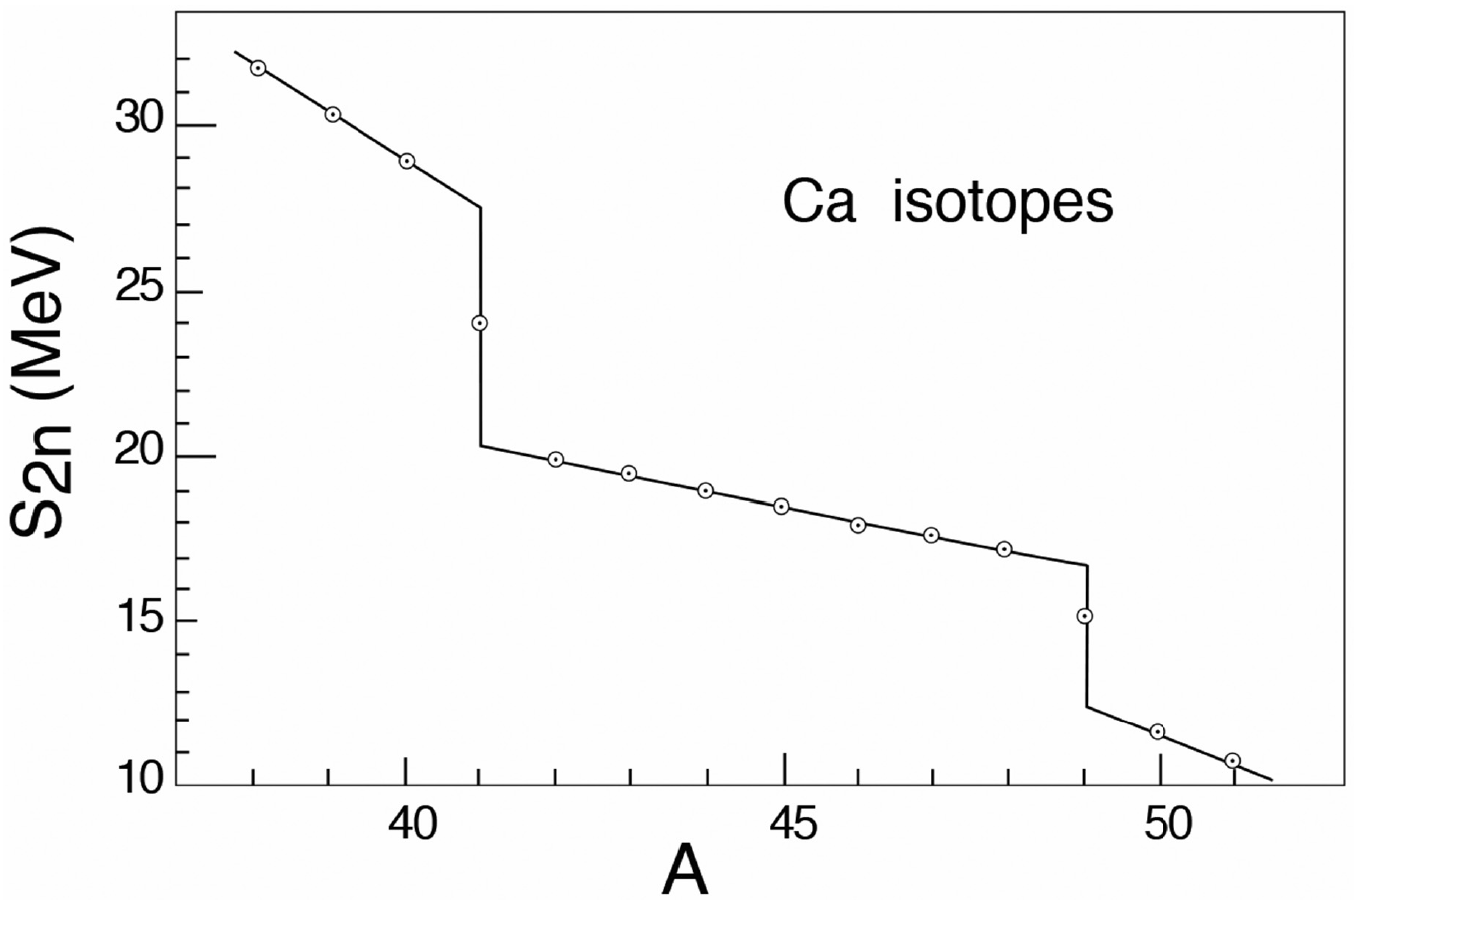
\includegraphics[width=\linewidth]{assets/2.1.4 S2n.png}
    \caption{Two-neutron separation energies. Data from \href{https://amdc.impcas.ac.cn/}{\ul{AMDC}} files. Fig. 1.11 \textit{Primer}.}
    \label{Sn}
\end{figure}

\subsection{Nuclear Shell Model}



\section{Prep Work for Surrey}
\begin{example}{1}{1-4: Binding Energy Calculations}
\textbf{The following table shows masses and binding energies in MeV for selected nuclei. Note that these are atomic masses. Data taken from AME2016.}
\begin{center}
\begin{tabular}{lll}
\toprule
{Isotope} & {$M(A,Z,N)$} & {$B(A,Z,N)$} \\
\midrule
n                   & 939.57    & 0       \\
$^{1}$H             & 938.78    & 0       \\
$^{2}$H             & 1876.12   & 2.22    \\
$^{4}$He            & 3728.40   & 28.30   \\
$^{5}$He            & 4668.70   & 27.56   \\
$^{6}$He            & 5606.56   & 29.27   \\
$^{8}$Be            & 7456.89   & 56.50   \\
$^{12}$C            & 11177.93  & 92.16   \\
$^{62}$Ni           & 57685.89  & 545.26  \\
$^{96}$Zr           & 89337.99  & 829.00  \\
$^{96}$Nb           & 89337.83  & 828.38  \\
$^{96}$Mo           & 89334.64  & 830.78  \\
$^{100}$Zr          & 93073.03  & 852.22  \\
$^{138}$Te          & 128480.49 & 1138.86 \\
$^{238}$U           & 221742.91 & 1801.69 \\
\bottomrule
\end{tabular}
\end{center}
\textbf{a.) How much gain in binding energy would be needed for \ce{^5{He}} to be bound in its ground state wrt disintegration into \ce{^4{He} + n}?}

The difference in binding energy between the products and reactants is positive so \ce{^4{He}} is more bound than \ce{^5{He} and energy is released}
\[B(\ce{^4{He}}) - B(\ce{^5{He}}) = 28.30-27.56=0.74\,\text{MeV}\]

\vspace{-1em}
\textbf{b.) How much gain in binding energy would be needed for \ce{^8{Be}} to be bound in its ground state wrt disintegration into \ce{^4{He} + ^4{He}}?}
\[2B(\ce{^4{He}}) - B(\ce{^8{Be}}) = 2(28.30)-56.50=0.1\,\text{MeV}\]

\vspace{-1em}
\textbf{c.) How much energy is needed to separate a neutron from \ce{^6He}?}
\[S_n = B(\ce{^6He})-B(\ce{^5He})=29.27-27.56=1.71\,\text{MeV}\]
\end{example}


\begin{example}{1}{1-6: Solar Energy Production}
\allbold{In the Sun, hydrogen fuses into \ce{^4He}. The age of the Sun is \(4.6 \times 10^9\) years and it has a mass of \(1.99 \times 10^{30}\) kg. The energy output of the Sun is \(4 \times 10^{20}\) MW.}

\allbold{a.) Using an electron mass of \(0.51\)MeV, how much energy is produced per atom of helium produced?}

The proton-proton chain has the net effect of converting four protons into one helium-4 nucleus whilst releasing two positrons.
\(4\ce{^1H} \to \ce{^4He}+2\ce{e^+}+2\nu_e + 2\gamma \)
\[(4m_p -m_{He})+4(m_e) = 4(938.78)-3728.4-2(0.51) = 25.7\,\text{MeV}\]
The two positrons then 
\allbold{b.) How many kilograms of hydrogen are being fused into helium per second?}

\textbf{c.) What percentage of its mass has been fused into helium so far?}

\allbold{d.) If the energy source of the Sun were chemical, how long would the Sun shine for the given energy output? Assume an energy yield of \(10\)eV per hydrogen atom.}
    
\end{example}

\begin{example}{2}{1-7: Fission of Uranium}
\allbold{Uranium can undergo fission, for example \ce{^{238}U \to ^{138}Te + ^{100}Zr}. How much energy is released per kilogram?}
\begin{equation*}
    \begin{split}
    \Delta B &= B(\ce{^{138}Te})+B(\ce{^{100}Zr})-B(\ce{^{238}U})\\
             &= 1138.86 + 852.22 - 1801.69\\
             &= 189.39 \,\text{MeV per fission}
\end{split}
\end{equation*}
In 1kg of \ce{^{238}U} there are of the order \(\frac{1000\text{g}}{238\text{gmol}^{-1}}\times N_A \approx 2.53 \times 10^{24}\text{ nuclei}\) of \ce{^{238}U}. So the energy released per kg is 
\[189.39 \times 2.53 \times 10^{24} = 4.79 \times 10^{26}\,\text{MeV kg}^{-1}\]
\end{example}

\begin{example}{1}{1-11: Electronic and Nuclear Binding Energy for Deuterium}
\textbf{For an atom of \ce{^2H}, what is the ratio of electronic binding energy to nuclear binding energy?}

The atomic ground state of \ce{^2H} is approximately \(13.6\) eV. Comparing this to the nuclear binding energy, \(2.22\) MeV:
\[\frac{13.6}{2.22 \times 10^6} \approx 6 \times 10^{-6} = 0.0006\%\]
\end{example}

\begin{example}[breakable]{3}{1-13: Finding the Line of Stability in Mass Parabolas}
\allbold{The Bethe-Weizs\"{a}cker formula for the binding energy of nuclei is expressed as
\[B(A,Z,N)=a_1A +a_2A^{2/3} + a_3\frac{Z^2}{A^{1/3}} + a_4\frac{(N-Z)^2}{A}\]
where the approximate values of the coefficients in MeV are \(a_1=15.68\), \(a_2=-18.56\), \(a_3=-0.717\) and \(a_4=-28.1\). The four terms are called the volume, surface, Coulomb and symmetry terms respectively. Note that there is no pairing term. Using \[M(Z, N) = Zm_p + Nm_n + Zm_e - B(Z, N)\] what would be the value of \(Z\) for the most stable isotope with:}

\allbold{a.) \(A=133\)? Compare with figure \ref{beta1}}

\allbold{b.) \(A=134\)? Compare with figure \ref{beta2}}

\allbold{c.) \(A=294\)?}

\allbold{d.) \(A=400\)?}

\allbold{Hint: Maximise \(B\) versus \(Z\) at constant \(A\) and substitute \(N=A-Z\) before starting}

Begin by casting \(B\) in terms of two variables. Substitute \(N=A-Z\).
\[B(A,Z) = a_1A +a_2A^{2/3} + a_3\frac{Z^2}{A^{1/3}} + a_4\frac{(A-2Z)^2}{A}\]
Then differentiate wrt \(Z\) at constant \(A\), set to zero to minimise.
\[\frac{\partial B}{\partial Z} = 2a_3\frac{Z}{A^{1/3}} - 4a_4\frac{(A-2Z)}{A} = 0\]
Rearrange to get \(Z_{min}\) in terms of \(A\).
\[Z_{min}(A) = \frac{2a_4 A}{a_3A^{2/3}+4a_4}=\frac{A}{\frac{a_3}{2a_4}A^{2/3}+2}\]
Which gives 

a.) \(Z_{min}(133) = 57.0\) MeV

b.) \(Z_{min}(134) = 57.4\) MeV

c.) \(Z_{min}(294) = 114.7\) MeV

d.) \(Z_{min}(400) = 148.6\) MeV
    
\end{example}

\begin{example}[breakable]{3}{1-14: Investigating the Bethe-Weizs\"{a}cker Formula}
\allbold{Explore the contribution of the four terms in the Bethe-Weizs\"{a}cker binding energy formula by setting, in turn, the parameters \(a_1\) to \(a_4\) to zero. How would such changes compress or expand the reach of the table of isotopes? Explore particularly the effects on the stability of the actinide isotopes and the relative stability of even-even, odd-\(A\) and odd-odd isotopes.}

Setting \(a_1 = 0\) removes the volume term, which represents the SNF between nearest 
\end{example}

\section{Nuclear Excitation Patterns}

\begin{example}{2}{2-5: Exploring \(\gamma\) Transition Energy Ratios}
\allbold{The ratios \(r_6\) and \(r_8\) are defined for nuclei which approximate an ideal rotor as \[r_6 = \frac{E(6^+_1) - E(4^+_1)}{E(2^+_1)} \quad\quad r_4 = \frac{E(4^+_1) - E(2^+_1)}{E(2^+_1)}\]}

\allbold{a.) Extend this study by defining \(r_8\)}
\[r_8 = \frac{E(8^+_1) - E(6^+_1)}{E(2^+_1)}\]

\allbold{b.) Obtain the rotor limit value for \(r_8\)}

Using \(E(I) \propto I(I+1)\) where \(I\) is the total angular momentum quantum number.
\[r_8 = \frac{8(8+1) - 6(6+1)}{2(2+1)} = 5\]
\allbold{c.) Using \ensdf for even-even rare earth and actinide nuclei around \ce{^{172}Yb} and \ce{^{242}Pu}, make a plot of \(r_8\) vs \(r_2\)}
\end{example}

\begin{example}[breakable]{2}{2-6: Nuclear Recoil Correction for Gamma Transitions}
\allbold{To obtain high precision on ratios of level energies as shown in figure \ref{r6_r4} it may be necessary to perform a correction to the gamma-ray energies observed in experiment as gamma-ray emission is a two-body process where the emitting nucleus recoils. So some small part of the transition energy is taken up by the recoil.}

\allbold{a.) Given that the photon's energy and momentum are related by \(E=pc\), make use of energy and momentum conservation to derive a formula for the nuclear recoil energy as a function of gamma-ray energy, \(E_\gamma\) and atomic mass, \(A\) of the recoiling nucleus.}

By conservation of momentum 
\[\begin{split}
    p_\gamma &= p_{\text{nuc}}\\
    \frac{E_\gamma}{c} &= p_{\text{nuc}}
\end{split}\]
So then the recoil energy of the nucleus will be
\[E_{\text{recoil}} = \frac{p_{\text{nuc}}^2}{2m_{\text{nuc}}} = \frac{E_\gamma^2}{2Ac^2}\]
where \(A\) is in amu. So for the units to work out, use \(c^2 = 931.5 \times 10^6 \,\text{eV/u}\).

\allbold{b.) Estimate the magnitude of the recoil correction for \(A=240\) and \(E_\gamma = 150\) keV.}
\[E_{\text{recoil}} = \frac{(150\times 10^3)^2}{2\times 240 \times 931.5 \times 10^6} = 0.05\,\text{eV}\]

\allbold{c.) Estimate the magnitude of the recoil correction for \(A=12\) and \(E_\gamma = 3213.79\) keV, \(E_\gamma = 4438.94\) keV. Note that these are the energies of \(\gamma\) rays de-exciting the Hoyle state in \ce{^{12}C}. Thus, give your estimate of the excitation energy of the Hoyle state and compare with the value given in \ensdf.}

For \(E_\gamma = 3213.79\) keV:
\[E_{\text{recoil}} = \frac{(3213.79\times 10^3)^2}{2\times 12 \times 931.5 \times 10^6} = 462.00\,\text{eV}\]

For \(E_\gamma = 4438.94\) keV:
\[E_{\text{recoil}} = \frac{(4438.94\times 10^3)^2}{2\times 12 \times 931.5 \times 10^6} = 881.38\,\text{eV}\]

So the total excitation energy of the Hoyle state is
\[3213.79+4438.94+0.462+0.88138 = 7654.07338\,\text{keV}\]
This matches the adopted level from the ENSDF, excerpt below.

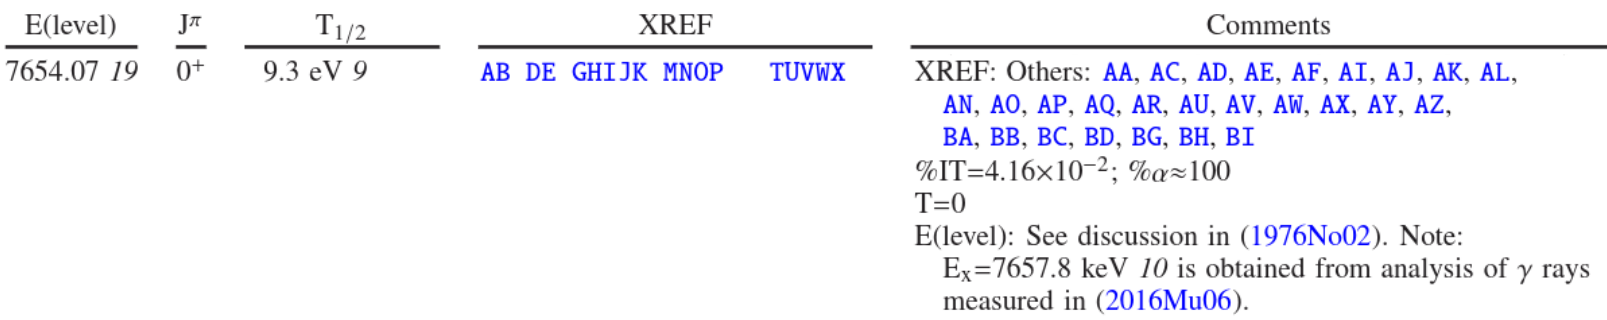
\includegraphics[width=\textwidth]{Hoyle.png}
\end{example}

\begin{example}{3}{2-11: Exploring the Nuclear Structure of \ce{^{152}Sm} with ENSDF Pages}
\allbold{Part 1: Levels}
Looking at adopted levels and gammas. First lot of tables gives the levels. Second lot gives the gammas that connect the levels.

First table gives energy, spin and parity, half life, flags (what reactions it was produced in) and comments. 
Easier to compute separation energies from the AMDC

If spin and parity, \(J^\pi\) is in brackets then its not firmly established. More XREF flags give more confidence. Footnotes contain info on how the data was manipulated but also assignments to different rotational bands. 

f are conversion coefficients, calculated with the bricc tool.

\allbold{Part 2: Matching Data to Levels}
22MeV deuteron scattering experiment. Unpblished so doesnt feature in the ensdf. Magnetic spectrograph used to analyse the scattered deuterons at a fixed angle of 60degrees with a high momentum bite setting. The data has FWHM energy resolution of about 3keV (much lower fidelity than possible by measuring gamma ray transitions with e.g. a high purity germanium detector). Consequently, the 1085 peak is seen as a single peak but is actually two closely spaced levels that aren't resolved 

As to how data is compiled in ENSDF, the energies of excited states are adopted from the highest precision measurements that are available. Usually \(\gamma\) ray transition measurements. For multiple sources, a weighted average of the most precise sources is adopted. To adopt a given excited state energy, a whole network of \(\gamma\) transition measurements is used, both de-exciting and populating a given level. Then, a least-squares fit is taken over the whole network. For \(\gamma\) ray energies with a very high precision (down to eV), then the recoil energy of the nucleus must be added to arrive at the transition energy. 
    
\end{example}


\section{Nuclear Deformation and Rotations}
\begin{example}{2}{3-1: }
\allbold{Below are the ground state rotational bands in \ce{^{242}Pu} and \ce{^{244}Pu} along with the excitation energies of the rotational states.} 

 \begin{minipage}[b]{0.48\textwidth}
        \centering
        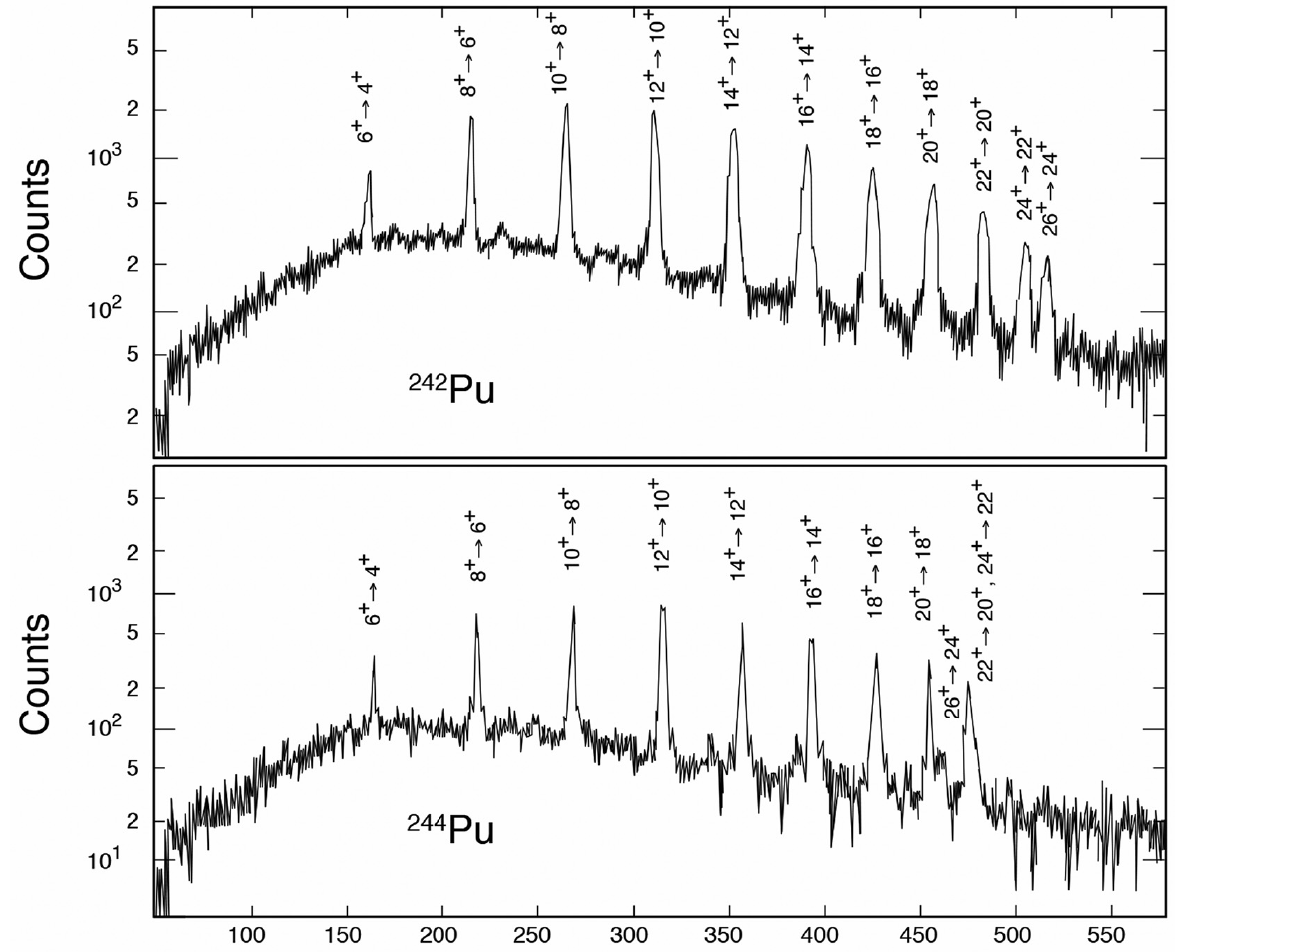
\includegraphics[width=\linewidth]{assets/Pu.png}
    \end{minipage}
    \hfill
    \begin{minipage}[b]{0.48\textwidth}
        \centering
        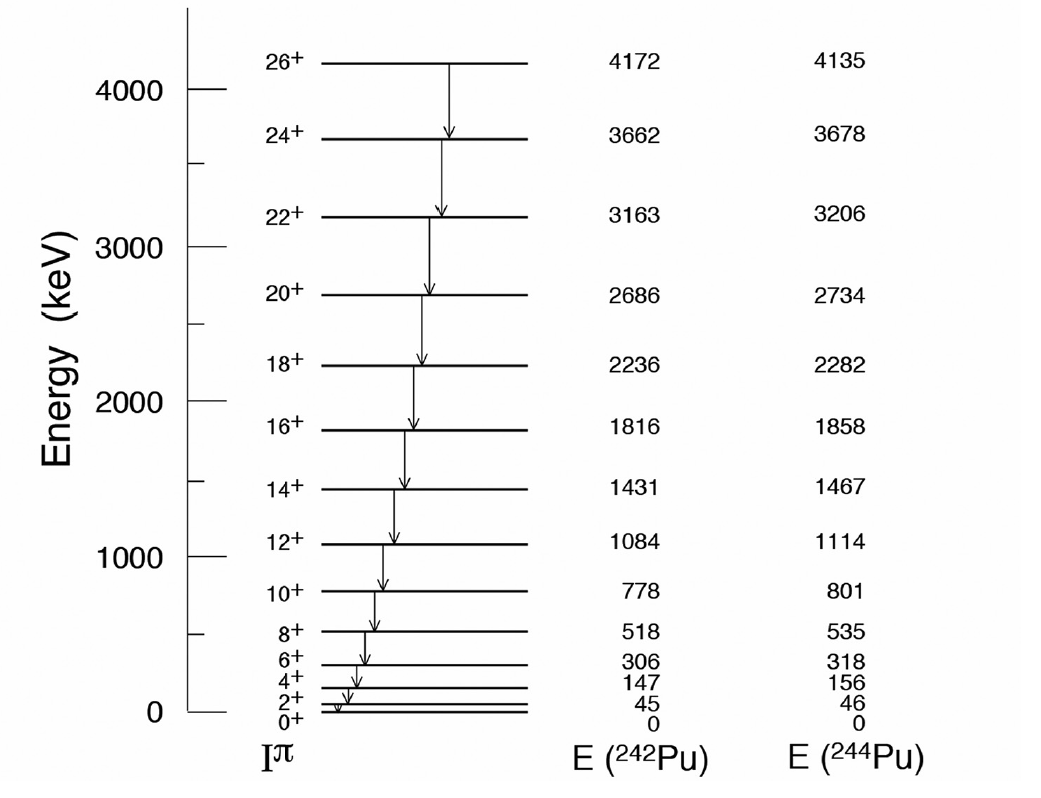
\includegraphics[width=\linewidth]{assets/Pu_levels.png}
    \end{minipage}



\allbold{Scale the excitation energies to that of \(2_1^+\) states i.e. divide the energies for \ce{^{242}Pu} by \(45\) and \ce{^{244}Pu} by \(46\). Having scaled the energies, plot the two bands as \(E(I_{\text{scaled}})\) vs \(I(I+1)\). Note that, while the energies look significantly different, when scaled they are nearly identical i.e. there is evidently some underlying universal rotational energy profile. This does not appear to have been recognised, but holds for the most strongly deformed ground-sate bands, extending into the rare earth region e.g. \ce{^{174}Yb}. Higher precision energy values can be used but this exercise captures the essence of the feature.}
\end{example}

\begin{example}{3}{3-6: Exploring the Nuclear Structure of \ce{^{175}Lu} with ENSDF Pages}
    
\end{example}

\section{Towards a Global View of Nuclear Structure}
\begin{example}{2}{4-4: J and M Coupling}
\allbold{Using the m scheme, deduce the possible couplings in terms of \(J\) and \(M\) for:}

\allbold{a.) Two identical fermions with \(j = 7/2\) e.g. coupling two \(\text{f}_{7/2}\) neutrons}

\allbold{b.) Three identical fermions with \(j = 7/2\) and obtained the allowed spins for the \(v=3\) states. Compare your result with information in figure \ref{Tb}.}

\allbold{c.) Two non-identical fermions with \(j = 7/2\) e.g. coupling an \(\text{f}_{7/2}\) proton and \(\text{f}_{7/2}\) neutron.}
    
\end{example}

\begin{example}{3}{4-10: Mirror Nuclei on the \(A=42\) Isobar}
\allbold{Make a comparison of the observed energies in \ensdf for the states in \ce{^{42}Ca}, \ce{^{42}Sc} and \ce{^{42}Ti} below 1600 keV as a side-by-side plot. Noting your answers to 4-4a, and that fact that \ce{^{42}_{20}Ca} and \ce{^{42}_{22}Ti} are a mirror pair, what can you conclude about the behaviour of the two valence nucleons in these \(A=42\) isobars?}
\end{example}

\begin{example}{3}{4-11: Exploring the Structure of \ce{^{207}Pb} and \ce{^{208}Pb} with ENSDF Pages}
\allbold{The following are notes from video exercises exploring different aspects of the structure of \ce{^{207}Pb} intended to encourage familiarity with identifying states adjoining the doubly magic nucleus, \ce{^{208}Pb}.}
\end{example}

\begin{example}{3}{4-6: Classification of the Lowest States in \ce{^{209}Bi}}
\allbold{Using \ensdf and information from the figures below, classify the lowest states in \ce{^{209}Bi} i.e. shell-model particle states, shell-model hole states and core-excited states coupled to shell-model particle states.}
\end{example}

\section{Simple Models of Nuclear Structure}

\begin{example}{2}{5-4: }
\allbold{Illustrate the difference in rotational energies for nuclei of mass \(A\) and \(A+1\) as depicted in plots of \(E_\gamma\) versus \(I_i\). Use the classical expression for the moment of inertia of a sphere.}
\end{example}
5-4

\section{Nuclear Spectroscopic Measurements}

\begin{example}{2}{6-1: Radii in the Bohr Model}
\allbold{The Bohr radius, \(a_0\) is the radius of an electron in the ground state of a Hydrogen atom \[a_0=\frac{4\pi \epsilon_0 \hbar^2}{m_e e^2}\] The corresponding radius for the first Bohr orbit for an element with higher \(Z\) is \[r_Z = \frac{a_0}{Z}\] a.) What would be the radius of the first Bohr orbit for a muon bound to \ce{^{150}_{60}Nd}?}

\allbold{b.) Is this orbit, on average, `inside' the nucleus?}

\allbold{c.) Using the concept of the first and second Bohr orbits, can the energy scale in the following spectra of muonic atom transitions be simply explained?}
    
\end{example}

\begin{example}{1}{6-4: Precision of a Penning Trap}
\allbold{The precision on nuclear masses which can be obtained depends on the number of ions in the measurement, \(N\), and the mass resolving power, \(R\): \[\frac{\delta m}{m}\propto \frac{1}{R\sqrt{N}}\]
The mass resolving power for a Penning trap is typically \(10^5\) for an observation time of \(100\) ms. This means that the isotope under study must be sufficiently long-lived to allow a measurement to be conducted for \(100\) ms. Estimate the number of ions that would need to be trapped to achieve a mass precision, \(\delta m/m=10^{-7}\)}
    
\end{example}

\begin{example}{3}{6-5: Lutetium-176}
\allbold{The isotope \ce{^{176}Lu} occurs naturally. Explain this in terms of expectations based on masses of \(A=176\) isobars and spins of states in \ce{^{176}Lu} and its neighbours.}
\end{example}

\begin{example}{1}{6-6: Isotopes of Uranium}
\allbold{The isotopes \ce{^{235}U} and \ce{^{238}U} both occur naturally. They possess relative natural abundances of \(0.7204\%\) and \(99.2742\%\), and half lives of \(7.04\times 10^{8}\) y and \(4.468\times 10^{9}\) y respectively. Assuming that these two isotopes were present in equal amounts when they were formed (in some coalescing binary neutron star pair) estimate how long ago that was. Compare this with the estimated age of the Earth, \(4.5\times 10^9\) y.}    
\end{example}


\begin{example}{1}{6-7: The Fraction of Plutonium in Uranium Ore}
\allbold{The longest lived isotope of plutonium is \ce{^{244}Pu} with a half life of \(8.13 \times 10^7\) y. Assuming that plutonium and uranium have similar mineral chemistry and were formed in equal amounts as in the scenario in 6-6, estimate the ratio \ce{^{244}Pu}/\ce{^{238}U} in uranium ore. Has this been investigated?}
\end{example}


Questions for David
What is the difference between an evaluation and a compilation of nuclear data

How do you choose the reference point for an isotope shift?
In the Bethe-Weizsacker formula (1-13) why is there no pairing term?

square vs curved brackets in the ensdf